% Leroviditve
\section{Felhasználói követelmények}
A felhasználói követelmények azokat a funkciókat írják le, amelyre a felhasználó szemszögéből szükség van. A rendszer két különböző felületet tartalmaz: felhasználói- és adminisztrátori felület, ezek pedig különböző felhasználói követelményekkel rendelkezhetnek, így ezeket külön-külön részletezzük.

\subsection{Felhasználói felület}
A felhasználói felület funkcióinak nagy része bejelentkezés nélkül használható, kivételt képez a jegyvásárlás és a jegyek listázása. A felhasználói felület követelményei a következők:

\begin{itemize}
  \item Legyen lehetőség utazást tervezni dátum, idő, kezdő- és célállomás alapján
  \item A talált járatok jelenjenek meg indulási idő szerinti növekvő sorrendben
  \item Legyen lehetősége a bejelentkezett felhasználónak jegyet vásárolni online a járatokra
  \item A rendszer jelenítse meg a buszok és megállók menetrendjeit
  \item A járatok útvonalait lehessen megtekinteni a térképen
  \item Térképen megtekinthetőek legyenek a megállók és szűrni is lehessen közöttük település vagy buszjárat alapján
  \item A rendszer biztosítsa a buszok valós idejű pozícióinak követését a térképen
  \item A QR-kódokkal ellátott megvásárolt jegyek megtekinthetőek legyenek bejelentkezés után
\end{itemize}

\subsection{Adminisztrátori felület}
Az adminisztrátori felület kizárólag bejelentkezéssel elérhető, új fiókokat pedig csak a cégek főnökei tudnak létrehozni, mindenki a saját busztársaságához. Itt regisztrációs lehetőség nincs, így meg lehet akadályozni az adminfelülethez való illetéktelen hozzáférést. A társult vállalatok főnökei a partnerség kezdetekor megkapják az admin jogú fiókjaikat, amelyekkel hozzáférnek a felülethez. Az adminfelületre vonatkozó követelmények:

\begin{itemize}
  \item A főoldalon emlékeztetők, értesítések, valamint statisztikák jelenjenek meg az eladott jegyek számáról, a megtett kilométerről és a bevételről, időintervallumok szerint csoportosítva
  \item Lehessen megtekinteni a megállók listáját, új megállókat hozzáadni térképen való megjelölés segítségével, valamit a meglévő megállókat szerkeszteni vagy törölni
  \item A rendszer listázza a buszjáratokat és biztosítson lehetőséget új járat létrehozására, meglévő járat szerkesztésére, valamint járatok törlésére
  \item A járatok indulási időpontjait lehessen megtekinteni, szerkeszteni és törölni is
  \item A buszjáratokhoz és az útvonalak különböző részeihez lehessen külön-külön jegyárat megadni
  \item A rendszer jelenítse meg a buszok listáját és biztosítson lehetőséget új busz hozzáadására, meglévő busz szerkesztésére, valamint buszok törlésére
  \item A buszokhoz hasonlóan lehessen kezelni az alkalmazotti fiókok listáját is
\end{itemize}

A rendszer funkcionalitását leíró használati eset diagram a \ref{fig:use-case} ábrán látható.

\begin{figure}[H]
  \centering
  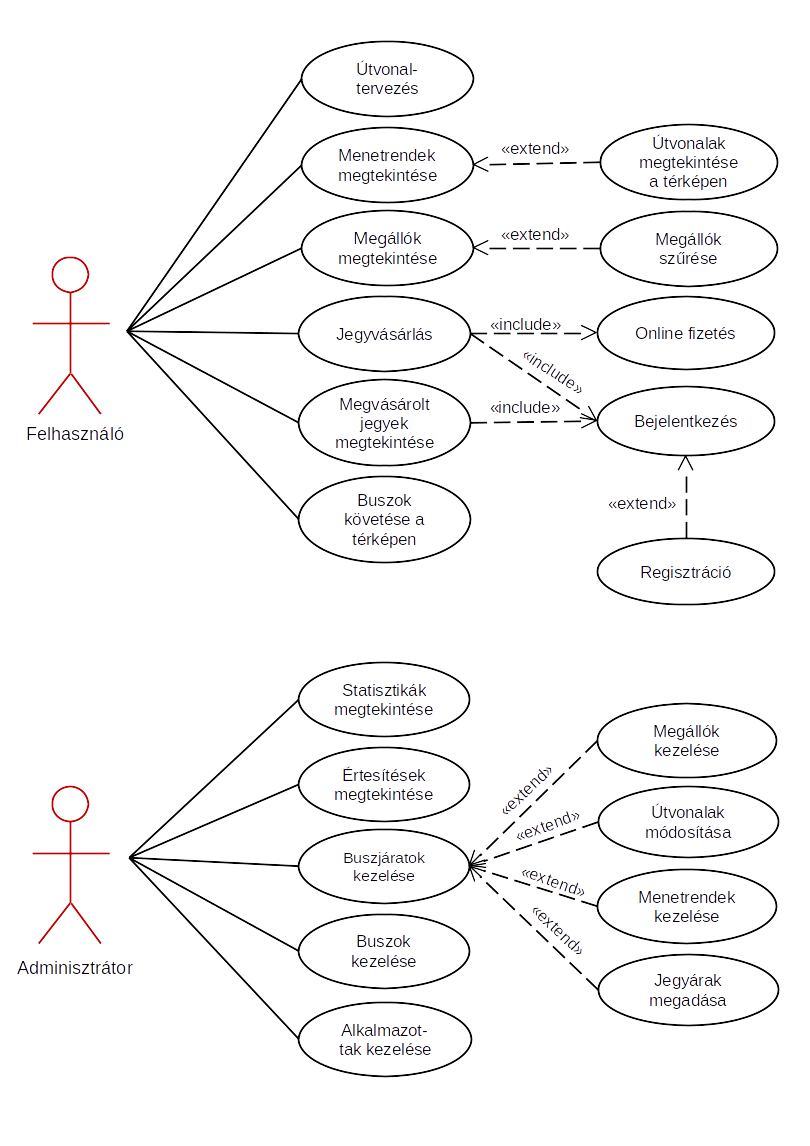
\includegraphics[height=0.92\textheight]{figures/use-case.png}
  \caption{Use-case diagram a felhasználók lehetőségeiről}
  \label{fig:use-case}
\end{figure}

\section{Rendszerkövetelmények}
\subsection{Funkcionális követelmények}

A funkcionális követelmények a felületen megjelenő funkciók működését írják le. Ezek foglalják össze, hogy adott bemenetre milyen kimenetet kell szolgáltatnia a rendszernek. A Bus4U esetében ezeket is két csoportba sorolhatjuk: felhasználói és adminisztrátori követelmények.

A felhasználói weboldalon és a mobilalkalmazásban bejelentkezés nélkül hozzá lehet férni a főoldalhoz, a menetrendekhez, a megállókhoz és az élő térképhez. Az egyetlen oldal, ami nem jeleníthető meg azonosítás nélkül az a jegyek oldal, innen a rendszernek át kell irányítania a bejelentkezési felületre. Itt biztosítani kell a regisztráció lehetőségét is, amennyiben a felhasználó még nem rendelkezik fiókkal. A regisztráció során a rendszer le kell ellenőrizzen minden megadott adatot, még az email tulajdonjogát is, azáltal hogy egy ellenőrző kódot küld a megadott email címre, amelyet be kell írni a felületen megjelenő szövegmezőbe. Sikeres regisztráció vagy bejelentkezés után a rendszernek minden adatot biztonságosan el kell mentenie, a jelszavat hash-elt formában és át kell irányítania a felhasználót a főoldalra.

A főoldalon lévő szövegmezőkben megadott adatok alapján a rendszernek le kell kérnie a szerverről néhány lehetséges járatot, amelyek indulnak az adott településről, adott időben, a megadott célállomásra. A megjelenített találatokhoz tartoznia kell egy jegyvásárlási lehetőségnek is, amelyben meg kell adni a jegyek számát és véglegesíteni kell a vásárlást. A jegyvásárlás is bejelentkezést igényel, így az azonosítatlan felhasználót a rendszer vásárlás előtt átirányítja a bejelentkezéshez. A sikeres vásárlást követi a jegy kódjának kigenerálása és elmentése. Ezek után a felhasználók megtekinthetik a megvásárolt jegyeket a Jegyek oldalon. A menetrendek oldalon a felhasználóknak lehetőségük van a buszok és megállók közötti választásra lenyíló listákból, amelyet követően a rendszer kilistázza az adott járat megállóhoz kötött időpontjait egy táblázatban. Ugyanitt a rendszernek lehetőséget kell biztosítania a buszok útvonalának megjelenítésére térképen. A megállók oldalon a felhasználóknak lehetőségük van az összes megálló megtekintésére térképen, valamint lenyíló listákat használva, a megállók szűrésére település vagy buszjárat alapján is. A térképen megjelölt megállókra való kattintás után meg kell jelennie az adott megálló adatainak egy boborékban. Az élő térkép oldalon a felhasználóknak lehetőségük van a buszok valós idejű pozícióinak követésére térképen. A megjelenített buszokat a rendszernek valós időben kell frissítenie, hogy a felhasználók pontos információkat kapjanak a buszok helyzetéről. A térképek alapfunkciói közé tartoznak a nagyítás, a kicsinyítés és a mozgatás. A felhasználónak látnia kell a saját pozícióját is a térképeken, amennyiben engedélyezte a helymeghatározáshoz való hozzáférést.

Az adminisztrátori weboldalon szükség van azonosításra, anélkül a rendszer minden oldalról átirányít a bejelentkezéshez. Itt a regisztráció nem lehetséges, így külső, admin szerepkörrel nem rendelkező felhasználók nem tudnak hozzáférni az adminisztrátori felülethez. A főoldalon található statisztikák között szerepel az eladott jegyek száma, a megtett kilométerek száma és a bevétel összege, időintervallumok szerint csoportosítva, táblázatos formában. Mivel minden busztársaságnak el kell legyenek különítve az adatai, ezért a szerver mindig a bejelentkezett adminhoz tartozó cég adataiból számolja ki a statisztikákat. A főoldalon a rendszernek meg kell jelenítenie az esetleges értesítéseket is, előugró "Toast" üzenetek segítségével. A megállók oldalon az adminisztrátoroknak lehetőségük van a megállók listázására, az ezekre való egyenkénti kattintás után pedig a szerkesztésükre is. Emellett megállók törlésére és új megállók hozzáadására is lehetőség van egy interaktív térkép segítségével. A térképre kattintva a hely koordinátáit a rendszer beilleszti az űrlapba, ahol meg kell adni még a megálló nevét és a címet is. Utóbbit, amennyiben elérhető, le kell kérnie a rendszernek a térképszolgáltatótól, hogy ezzel is gyorsítsa a folyamatot. A járatok oldalon az adminisztrátoroknak lehetőségük van a buszjáratok kiválasztására egy lenyíló menüből, ezt követően pedig meg kell jelennie a járatszerkesztő űrlapnak. Ugyanitt lehetőség lesz járatok hozzáadására és törlésére is. A menetrendek oldalon az adminisztrátoroknak lehetőségük van a járatok indulási időpontjainak és jegyárainak megtekintésére, szerkesztésére és törlésére. Az órarendek bevitelét le kell lehessen bontani napokra, ezeket pedig dinamikusan megjeleníteni, hogy minél kevesebb helyet foglaljon az oldalon. A buszok és alkalmazottak oldalakon a rendszernek biztosítania kell egy egységes felületet, amelyben lehetőség nyílik az elemek listázására, új elemek hozzáadására, meglévő elemek szerkesztésére és ezek törlésére is. A buszoknál fontos megadni az útadó, biztosítás és műszaki vizsga időpontjait, mert a rendszer ezek alapján fog emlékeztetőket megjeleníteni a felületre való belépések alkalmával. Az alkalmazottaknál meg kell adni a nevet, a beosztást és a telefonszámot, valamint az emailt és a jelszót is. Utóbbiak az alkalmazott bejelentkezéséhez lesznek szükségesek, így a rendszernek ellenőriznie kell őket.

\subsection{Nem funkcionális követelmények}
\subsubsection{Szervezéssel kapcsolatos követelmények}

\begin{itemize}
  \item Programozási nyelvek: Dart, HTML, CSS, JavaScript
  \item Keretrendszerek: Flutter, Vue.js
  \item IDE: Visual Studio Code
  \item Verziókövetés: Git és GitHub
  \item Webhost: Netlify
  \item Csoportos kommunikáció: Slack
\end{itemize}

\subsubsection{Termékkel kapcsolatos követelmények}

A felhasználói weboldal és az admin felület használatához egy modern, internetezésre alkalmas eszközre van szükség, a térképfunkciók teljes kihasználásához engedélyezni kell a helymeghatározást. A Vue.js keretrendszer minimum a JavaScript ES2016-os verzióját követeli meg, viszont a Vuetify komponensek miatt ajánlott a 2021 után kiadott böngészőverziók használata\footnote{Vuetify böngésző támogatás: \url{https://vuetifyjs.com/en/getting-started/browser-support/}}:
\begin{itemize}
  \item Chromium (Chrome, Edge, Opera, Brave) >= 90
  \item Firefox >= 88
  \item Safari >= 15
\end{itemize}

Az mobilapplikáció használatához szükség van egy okostelefonra vagy tabletre,
amelyen minimum Android 5.0 vagy iOS 8.0 operációs rendszer fut. Fontos hogy legyen
rajta internet elérés (3G,4G,5G vagy Wi-Fi), legalább 120MB szabad tárhely és 516-1024 MB szabad memória. Itt is ajánlott a helymeghatározás (GPS) engedélyezése, hogy a térképfunkciók helyesen működjenek.
